\section{Process view}

Ingen af systemets centrale dele gør brug af tråde. Men systemet er opbygget således at afvikling af drone, website og server kan betragtes som 3 samtidige processer. Alle 3 dele bruges sideløbende i runtime og imellem dem flyder løbende data.

For systemets bruger ser det ud som om al information går direkte fra website til drone eller omvendt. Men reelt set er websitet og drone aldrig i direkte kontakt med hinanden. I stedet går al kommunikation til og fra serveren, som fungerer som et kommunikationslag. 

\vspace{-5pt}
\begin{figure}[H]
	\centering
	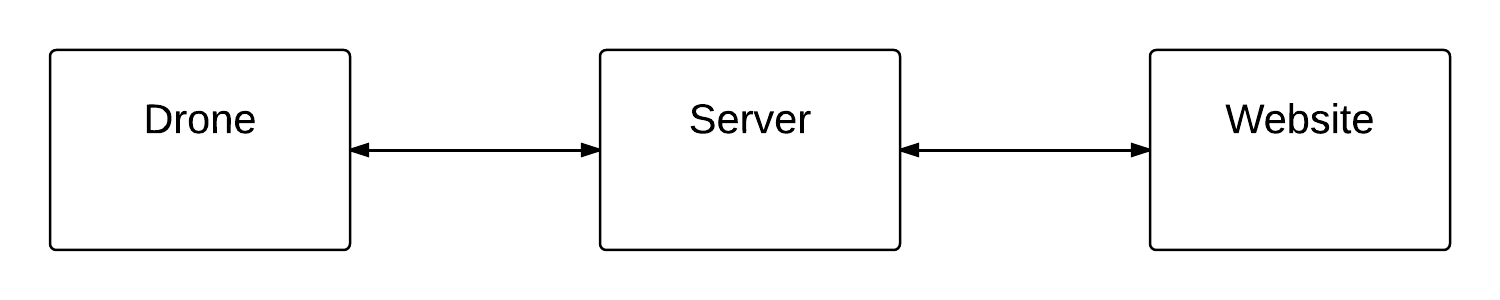
\includegraphics[width=0.7\textwidth]{Billeder/process_view}
	\vspace{0cm}
	\caption{Process view}
	\label{fig:process_view}
\end{figure}

\textbf{Server}\\
Serveren er passiv, hvilket betyder den aldrig tager initiativ til udveksling af data. Serveren foretager ingenting på egen hånd, den står i stedet og venter på at blive igangsat af drone eller website. 
 
\textbf{Drone} \\
I drone processen håndteres al styring af drone og kommunikation mellem drone og server. Når dronen er tændt og 3G/GPS modulet initialiseret, opdaterer dronen med få minutters interval egen GPS position for efterfølgende at sende serveren information om positionen. Desuden kontrollerer dronen løbende om der er en ny flyveopsætning tilgængelig på serveren. Hvis der er en ny flyveopsætning tilgængelig hentes den, og en ny flyvning påbegyndes. 

\textbf{Website}\\
Mellem server og website er der lavet en socket connection. Det betyder at indholdet af websitet opdateres hver gang der kommer nyt indhold på serveren. Desuden bruges websitet når systemets bruger ønsker at lave nye flyveopsætninger eller opdatere de nuværende.\\


Der er lagt megen energi i at designe og bygge systemet på en vis der tillader udvidelser og tilføjelser. Dels kan server nemt tilgås af flere forskellige websites og desuden kan websitet nemt håndtere flere droner og client’er samtidig.